\documentclass[french, 12pt]{article}%

\usepackage[utf8]{inputenc}  
\usepackage[francais]{babel}
\usepackage{appendix}
\usepackage{pdfpages} 
\usepackage{eurosym}
%\usepackage[T1]{fontenc}

%%%%%%%%%%%%%%%%%%%%%%%%%%%%%%%%%%%%%%%%%%%%%%%%%%%%%%%%%
\newcommand{\itemE}{\item[$\bullet$]}
\newcommand{\titreSeq}{Introduciton ZentithCIEL}
\newcommand{\lycee}{Lycée Brocéliande}
\newcommand{\classSeq}{CIEL }
\newcommand{\matiereSeq}{IR}      
\newcommand{\numSeq}{Formation}
\newcommand{\numAct}{Wifi-Intro}
\newcommand{\objSeance}{Présenter la salle de concert ZenithCIEL}

\newcommand{\moySeq}{\begin{itemize}	
\itemE Esp32
\itemE IDE de programmation ESP32
\itemE Machine windows
\end{itemize}}

\newcommand{\compSeq}{\begin{itemize}
\item  
\end{itemize}}
%%%%%%%%%%%%%%%%%%%%%%%%%%%%%%%%%%%%%%%%%%%%%%%%%%%%%%%%%%

%%%%%%%%%%%%%%%%%%%%%%%%%%%%%%%%%%%%%%%%%%%%%%%%%%%%%%%%
%%%%Algo
\usepackage[linesnumbered, french]{algorithm2e}
\SetKwFor{For}{Pour}{faire}{fin}
\SetKwFor{While}{Tant que}{faire}{fin}%
\SetKw{KwTo}{à}
\SetKw{KwPas}{par pas de}
\SetKw{KwRet}{Retourne}
\SetKwProg{Fn}{Fonction }{ arguments }{fin}
\SetKwRepeat{Repeat}{Répéter}{jusqu'à}%
\SetKwIF{If}{ElseIf}{Else}{Si}{alors}{Sinon si}{Sinon}{Fin}

\usepackage{listings} %%%%Présenration code source
\lstset{language=C++,
    %numbers=left,
   %stepnumber=1,
    showstringspaces=false,
    tabsize=1,
    breaklines=true,
    breakatwhitespace=false,
    basicstyle=\footnotesize,
    keywordstyle=\color{blue}\footnotesize,
    stringstyle=\color{red}\footnotesize,
    commentstyle=\color{magenta}\footnotesize,
    morecomment=[l][\color{magenta}]{\#}
    }
\lstdefinestyle{commande}{
  basicstyle=\ttfamily\footnotesize,
  keywordstyle=\color{blue},
  commentstyle=\color{gray},
  %numbers=left,
  %numberstyle=\tiny\color{gray},
  numbersep=5pt,
  breaklines=true,
  frame=single,
  backgroundcolor=\color{lightgray!10}
  %captionpos=b,
  %caption=\lstname  
}
%\usepackage[T1]{fontenc}


% Margins
\topmargin=-0.45in
\evensidemargin=0in
\oddsidemargin=0in
\textwidth=6.5in
\textheight=9.0in
\headsep=0.25in 


\linespread{1.1} 
\usepackage{amsmath}%
\usepackage{amsfonts}%
\usepackage{amssymb}%
\usepackage{graphicx}
\usepackage{lastpage}
\usepackage{enumitem}

%\usepackage[T1]{fontenc}    
\usepackage{multirow}
\usepackage{lscape}
\usepackage[colorlinks = true,
            linkcolor = blue,
            urlcolor  = blue,
            citecolor = blue,
            anchorcolor = blue]{hyperref}
\usepackage{array}
\usepackage{mwe}
%-------------------------------------------
\newtheorem{theorem}{Theorem}
\newtheorem{summary}[theorem]{Summary}
\newenvironment{proof}[1][Proof]{\textbf{#1.} }{\ \rule{0.5em}{0.5em}}



\usepackage{xcolor}

\usepackage{colortbl}
\setlength{\doublerulesep}{\arrayrulewidth}
%-------------------------------------------
%%%%%%%%%%%%%%%%%%%%%%%%%%%%%%%%%%%%%%%%%%%%%
\usepackage[framemethod=tikz]{mdframed}
\usepackage{tikz, xcolor, lipsum}
\makeatletter
\mdfsetup{skipabove=\topskip,skipbelow=\topskip}

\tikzset{titre_bleu_snir/.style =
	{draw=vert_capet, line width=1.5pt, fill=white,
	rectangle, rounded corners, right,minimum height=2em}}
\newcommand{\titreencadre}{Titre}
\makeatletter
\mdfdefinestyle{encadrestyle}{%
	linewidth=1.5pt,roundcorner=5pt,linecolor=vert_capet,
	apptotikzsetting={\tikzset{mdfbackground/.append style ={%
		fill=white}}},
	frametitlefont=\bfseries,
	singleextra={%
		\node[titre_bleu_snir,xshift=2em] at (P-|O) %
			{~\mdf@frametitlefont{\titreencadre}\hbox{~}};},
	firstextra={%
		\node[titre_bleu_snir,xshift=2em] at (P-|O) %
		{~\mdf@frametitlefont{\titreencadre}\hbox{~}};},
	}
\mdfdefinestyle{encadresanstitrestyle}{%
	linewidth=1.5pt,roundcorner=5pt,linecolor=vert_capet
	apptotikzsetting={\tikzset{mdfbackground/.append style ={%
		fill=yellow!20}}},
	}

\newenvironment{encadre}[1]{\renewcommand{\titreencadre}{#1}
	\begin{mdframed}[style=encadrestyle]
	\vspace{0.5\baselineskip}
	}{%
	\end{mdframed}}

\newenvironment{encadresanstitre}{
	\begin{mdframed}[style=encadresanstitrestyle]
	}{%
	\end{mdframed}}
\makeatother
\usepackage{colortbl}
\definecolor{vert_capet}{RGB}{191,255,191}	
\definecolor{bleu_snir}{RGB}{191,255,191} %%{101,191,179}	
\setlength{\doublerulesep}{\arrayrulewidth}
%-------------------------------------------
\usepackage{comment}
%%%%%%%%%%%%%%%%%%%%%%%%%%%%%%%
\newif\ifPROF

%\def\PourProf{0}
\ifdefined\PourProf
  \PROFtrue
  \newenvironment{corr}{\begingroup \color{red}}{\normalcolor \endgroup}
\else
  \PROFfalse
  \newenvironment{corr}{\begingroup \color{white}}{\normalcolor \endgroup}
\fi
%\PROFtrue

%%%%%%%%%%%%%%%%%%%%%%%%%%%%%%%%%%%%




%%%Note et pied de page
\usepackage{fancybox}
\usepackage{fancyhdr}
\usepackage[a4paper,margin=2.5cm,bottom=2cm,headheight=2cm]{geometry}
\pagestyle{fancy}
\fancyhead[R]{
\includegraphics[scale=0.3]{logo_CIEL.png}}
\fancyhead[C]{Prénom}
\fancyhead[L]{Nom}
\fancyfoot[C]{Page \thepage/\pageref{LastPage}}
\fancyfoot[L]{\classSeq ~\matiereSeq}
\fancyfoot[R]{Seq \numSeq  ~ Act \numAct}
\renewcommand{\headrulewidth}{1pt}
%%%Note et pied de page 



\begin{document}

\title{\titreSeq\\
 
\includegraphics[scale=0.5]{logo_CIEL.png}\\
}
\author{\lycee}
\date{}%\today}
%\maketitle

\noindent\begin{tabular}{!{\vrule width 1.5pt}m{0.7\linewidth}!{\vrule width 1.5pt}m{0.2\linewidth}!{\vrule width 1.5pt}}
\hline\hline
\cellcolor{bleu_snir}
\begin{center}
	\Large\textbf{\titreSeq}  
\end{center}
  & 

\begin{minipage}{1.0\linewidth}
  \vspace*{0.1cm} 
\centering
\includegraphics[scale=0.2]{logo_lycee.jpg}

{\tiny\today}
  \vspace*{0.1cm} 
\end{minipage}\\ \hline\hline

\multicolumn{2}{!{\vrule width 1.5pt}l!{\vrule width 1.5pt}}{
\begin{minipage}{14cm}
\vspace*{0.1cm} 
\textbf{Objectif} : \objSeance
\vspace*{0.1cm} 
\end{minipage}} \\ \hline\hline

\multicolumn{2}{!{\vrule width 1.5pt}l!{\vrule width 1.5pt}}{
\begin{minipage}{14cm}
\vspace*{0.1cm} 
\textbf{Moyens} : 
\moySeq
\vspace*{0.1cm} 
\end{minipage}} \\ \hline\hline
%
%\multicolumn{2}{!{\vrule width 1.5pt}l!{\vrule width 1.5pt}}{
%\begin{minipage}{14cm}
%\vspace*{0.1cm}
%\tiny
%Compétences attendues :
%\compSeq
%\vspace*{0.1cm}
%\end{minipage}}
%\normalsize \\ \hline\hline
\end{tabular}

%%%%%%%%%%%%%%%%%%%%%%%%%%%%%%%%%%%%%%%%%%%%%%%%%%%%%%%%%%%%%%%%%%%%%%%%%%%%%%%%
\vspace{0.25cm}

%%%%%%%%%%%%%%%%%%%%%%%%%%%%%%%%%%%%%%%%%%%%%%%%%%%%%%%%%%%%%%%%%%%%%%%%%%%%%%%%%%%%%%%%%%%%%%%
%%%%%%%%%%%%%%%%%%%%%%%%%%%%%%  DEBUT %%%%%%%%%%%%%%%%%%%%%%%%%%%%%%%%%%%%%%%%%%%%%%%%%%%%%%%%%
%%%%%%%%%%%%%%%%%%%%%%%%%%%%%%%%%%%%%%%%%%%%%%%%%%%%%%%%%%%%%%%%%%%%%%%%%%%%%%%%%%%%%%%%%%%%%%%
\section{Présentation de ZenithCIEL}
ZenithCIEL est une grande salle de concert située à Guer - 56, capable d'accueillir de milliers de spectateurs. Conçue pour offrir une expérience unique, elle dispose d'une infrastructure moderne et d'une équipe dédiée composée de techniciens et d'ingénieurs du son. Des stars internationales y ont réalisé de magnifiques spectacles : 

\begin{minipage}{0.4\linewidth}
\begin{itemize}
\itemE Johnny Dion
\itemE Céline Hallyday
\itemE Two Direction
\itemE...
\end{itemize}
\end{minipage}
\begin{minipage}{0.6\linewidth}
\begin{center}
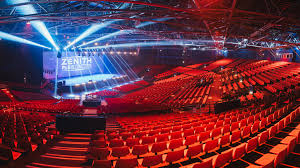
\includegraphics[scale=0.6]{./ressource/salleConcert.png}
\end{center}
\end{minipage}

\section{Organisation de ZenithCIEL}
ZenithCIEL est organisé en trois services principaux : gestion des clients, gestion des artistes et management de la salle.

\subsection{Gestion des clients}
Cette section est dédiée à la relation avec les spectateurs et couvre les aspects suivants :
\begin{itemize}
    \itemE \textbf{Réservations des places :} Les spectateurs peuvent réserver leurs places en ligne via une plateforme dédiée, avec des options de choix des sièges.
    \itemE \textbf{Paiements en ligne :} Un système de paiement sécurisé est en place pour faciliter les transactions.
    \itemE \textbf{Proposition de concerts :} La plateforme propose une sélection de concerts adaptée aux préférences des utilisateurs grâce à des recommandations personnalisées.
\end{itemize}

\subsection{Gestion des artistes}
La gestion des artistes est essentielle pour assurer une programmation fluide et des conditions optimales pour les performances. Elle inclut :
\begin{itemize}
    \itemE \textbf{Planning des artistes :} Un calendrier détaillé est maintenu pour coordonner les disponibilités des artistes et programmer les répétitions.
    \itemE \textbf{Paiement des artistes :} Les cachets des artistes sont gérés via un système automatisé.
    \itemE \textbf{Programmation des salles :} Les salles sont attribuées et préparées en fonction des besoins spécifiques des artistes.
\end{itemize}

\subsection{Management de la salle}
Pour garantir une expérience optimale, ZenithCIEL met l'accent sur la gestion de ses installations :
\begin{itemize}
    \itemE \textbf{Gestion des indicateurs de qualité de l'air intérieur :} Un système avancé surveille et régule la qualité de l'air pour le confort et la sécurité des occupants.
    \itemE \textbf{Système de gestion de la qualité :} Des normes strictes sont appliquées pour maintenir la qualité globale des prestations.
    \itemE \textbf{Gestion du son et des lumières :} Une équipe dédiée assure la configuration et le contrôle des équipements sonores et lumineux pour chaque événement.
    \itemE \textbf{Gestion des entrées et sorties :} Un système de contrôle des accès garantit une circulation fluide et sécurisée des spectateurs et des artistes.
\end{itemize}

\section{Infrastructure matérielle et gestion des données}
ZenithCIEL repose sur une infrastructure informatique robuste pour gérer ses services. Voici les principaux éléments :
\subsection{Serveurs internes}
\begin{itemize}
    \itemE \textbf{Gestion des réservations clients :} Un système de gestion interne gère les réservations et les préférences des spectateurs.
    \itemE \textbf{Gestion des clients :} Une base de données sécurisée conserve les informations des utilisateurs.
    \itemE \textbf{Gestion des artistes et des plannings :} Un logiciel interne permet de planifier et de suivre les activités des artistes.
\end{itemize}

\subsection{Serveurs externes}
\begin{itemize}
    \itemE \textbf{Gestion bancaire :} Les paiements en ligne et les transactions financières sont externalisés auprès de prestataires spécialisés pour garantir un traitement sécurisé et conforme.
\end{itemize}

\subsection{Management de la salle}
\begin{itemize}
    \itemE Tous les équipements liés au son, aux lumières, à la qualité de l'air et au contrôle des entrées/sorties sont gérés par des serveurs internes
    \itemE Les capteurs de qualité de l'air (CO2 et température) communiquent en Wifi avec le serveur.
    \itemE Ces systèmes ont été initialement installés par des prestataires, mais leur gestion au quotidien est assurée par l'équipe interne de ZenithCIEL.
\end{itemize}


\section{Résumé de ZenithCIEL}
ZenithCIEL est une salle de concert innovante et polyvalente, soutenue par une infrastructure technique de pointe et une organisation rigoureuse. Grâce à cette combinaison de technologies et de services, elle offre une expérience exceptionnelle pour les spectateurs et les artistes. \footnote{merci l'IA pour cette belle description}

\section{Votre travail}

Vous allez dans un premier temps réaliser avec la méthode EBIOS une analyse de risque pour évaluer et corriger si beoins les risques liés à la cybersécurité. 

Si des risques sont identifiés, vous essaierez de réduire leur impact ou leur vraisemblance. 


\ifPROF
\begin{center}
\includegraphics[scale=0.5]{./ressource/présentationAcitivte.png}
\end{center}
\fi	


\end{document}
